%\chapter[Name in the PDF menu]{Name in the text (and index)}
\chapter{Experimental setup}
\label{sec:experiment}
This thesis uses data obtained through the CMS experiment, which is one of the four major experiments operating at the CERN Large Hadron Collider (LHC).
CERN, the European Organisation for Nuclear Research, was founded in 1954 by a consortium of 12 European countries and its original programme was the study of atomic nuclei.
Over the time, CERN's scientific endeavours have extended in parallel with the understanding of matter, and its current main research area is particle physics: the fundamental constituents and the forces that govern them.
To investigate fundamental interactions, particles are accelerated through a chain of particle accelerators culminating (at the present day) with the LHC.
The collision products are observed and recorded by particle detectors, such as the CMS experiment.

\section{The Large Hadron Collider}
The Large Hadron Collider (LHC) \cite{CERN-AC-93-03-LHC}, situated at the European Organisation for Nuclear Research (CERN) in Geneva, is a two-ring superconducting accelerator designed for high-energy particle collisions.
It operates within a circular underground tunnel 26.7~kilometres long, originally excavated to accommodate the LEP electron-positron collider, operating from 1989 to 2000.

The LHC accelerates two counter-rotating beams, primarily composed of protons but also capable of collision with heavy nuclei like lead (Pb) at varying energies.
The acceleration process involves a sequence of pre-accelerators, shown in Figure \ref{fig:CERNaccelerators}.
The protons are isolated from a duoplasmatron source, accelerated through Linac2 to 50\MeV, further pushed in the Proton Synchrotron Booster (PSB) to 1.4\GeV, accelerated to 25\GeV in the Proton Synchrotron (PS), and finally reach an energy of 450\GeV in the Super Proton Synchrotron (SPS) before entering the LHC rings.

LHC was designed to accelerate protons up to 7\TeV ($\sqrt{s} = 14\TeV$),
and has successfully operated at 3.5 and 4\TeV during \Run1 (2009--2013),
at 6.5\TeV during \Run2 (2015--2018) and 6.8\TeV during the ongoing \Run3 (started in 2022).
Operation at 7\TeV is scheduled for the upcoming High Luminosity LHC (HL-LHC) after the so called ``Long Shutdown 3'', which is foreseen for 2026.

\begin{figure}[htb]
\begin{center}
\includegraphics[width=0.85\textwidth]{Figures/CCC-v2017.png}
\end{center}
\caption{The CERN accelerator complex \cite{OPEN-PHO-ACCEL-2016-009}. The protons start from the LINAC2 and are accelerated by the Booster, the PS and SPS before reaching the LHC.}
\label{fig:CERNaccelerators}
\end{figure}

The LHC's design incorporates various types and sizes of magnets, each serving specific functions: dipole magnets bend the beams,
quadrupole magnets focus the beams in the horizontal and vertical plane,
and sextupole magnets compress the beams closer to the intersection points to increase the likelihood of particle interactions.
This highly sophisticated accelerator operates at temperatures as low as 1.9 K (-271.25 $^\circ$C) by utilizing superfluid helium to cool and maintain the superconducting electromagnets capable of producing magnetic fields of 8.65 T.

Proton bunches in the LHC are spaced by 25 ns and cross at a rate of 40 MHz.
The nominal number of protons per bunch is $N_b = 12 \times 10^{11}$ and the nominal number of bunches is $2808$.
The LHC design luminosity of \LHigh was achieved in 2016, and by the end of 2017 it reached twice this value.
The parameters used by LHC in each year of \RunII{} are reported in Table~\ref{tab:LHCparamsRun2}.

The data recorded by the CMS detector\footnote{
These figures refer to the runs suitable for physics, \eg excluding commisioning, calibrations and special runs, and account for the detector deadtime.
The total luminosity delivered by LHC during the 2016--2018 period is is $159.3\fbinv$.}
corresponds to an integrated luminosity of $36.3\fbinv$ in 2016, $41.5\fbinv$ in 2017 and $59.8\fbinv$ in 2018,
for a total of $137.6\fbinv$.

\begin{table}
  \caption{The main LHC machine parameters for the data production years in \RunII{} compared to the design beam configuration~\cite{CERN-2004-003}.
  The mean number of interactions per bunch crossing (\pileup) denoted with $<\mu>$ is taken from References~\cite{CMS-LUM-17-003, CMS-LUM-17-004, CMS-LUM-18-002}.
  To compare the \pileup{} conditions at different values of the centre-of-mass-energy, the theoretical prediction of the pp inelastic cross-section derived with
  \PYTHIA~\cite{Sjostrand:2015} is used, \ie $\sigma^{13\TeV}_{\text{incl.}}(\Pp\Pp) = 80.0\unit{\text{mb}}$.}
  \label{tab:LHCparamsRun2}
  \centering
  \begin{tabular}{l c c c c}
    \toprule
    Parameter                & Design & 2016 & 2017 & 2018\\
    \midrule
    Beam energy [$\TeV$]     &     7  &  6.5 &  6.5 &  6.5\\
    %% Bunch spacing [ns]      &    25  &  25  & 25   & 25  \\
    $N_p^{bunch}\ [10^{11}]$ &  1.15  & 1.1  & 1.15 & 1.15\\
    $N_{bunches}$            &  2808  & 2220 & 2556 & 2556\\
    $\mathcal{L}_{peak}\ [10^{34}\cm^{-2}\text{s}^{-1}]$ & 1 & 1.4 & 2.06 & 2.01\\
    $<\mu>$                  &    20  &   27 &   38 &   37\\
    \bottomrule
  \end{tabular}
\end{table}

\section{The Compact Muon Solenoid experiment}
The Compact Muon Solenoid (CMS) is one of the two general purpose detectors operating at the LHC.
It is installed in a 100-meter deep cavern situated in the proximity of the French village of Cessy.
The detector was designed to cover a broad scope of physics analyses at the TeV scale, ranging from precision measurements of the electroweak observables to Beyond Standard Model (BSM) searches.
The main feature of the CMS experiment is its superconducting solenoid magnet with 6\usep m internal diameter and 12.5\usep m length, which provides a highly homogeneous magnetic field of 3.8\usep T inside, and around 2\usep T in the steel return yoke.
The high field intensity allows the overall apparatus to be compact, compared to other experiments such as ATLAS, the other LHC general purpose detector.
CMS is 21.6 meters long, 14.6 meter wide and weights 14000 tonnes.

The high bending power is needed to accurately measure the momentum of charged particles up to 1\TeV.
The fine granularity of the CMS detector over a large geometrical coverage allows achieving excellent muon identification and momentum resolution.
The other detector features are the high resolution of the electromagnetic and hadronic calorimeters, and the excellent tracking and vertexing capability.

In order to distinguish between particle signatures, and to provide the most precise measurements of their properties,
CMS was built with concentric layered structure, each subdetector layer targeting a certain interaction type.
A schematic diagram of CMS and its subdetectors is illustrated in Figure \ref{fig:CMSslice}.

\begin{figure}[htb]
\begin{center}
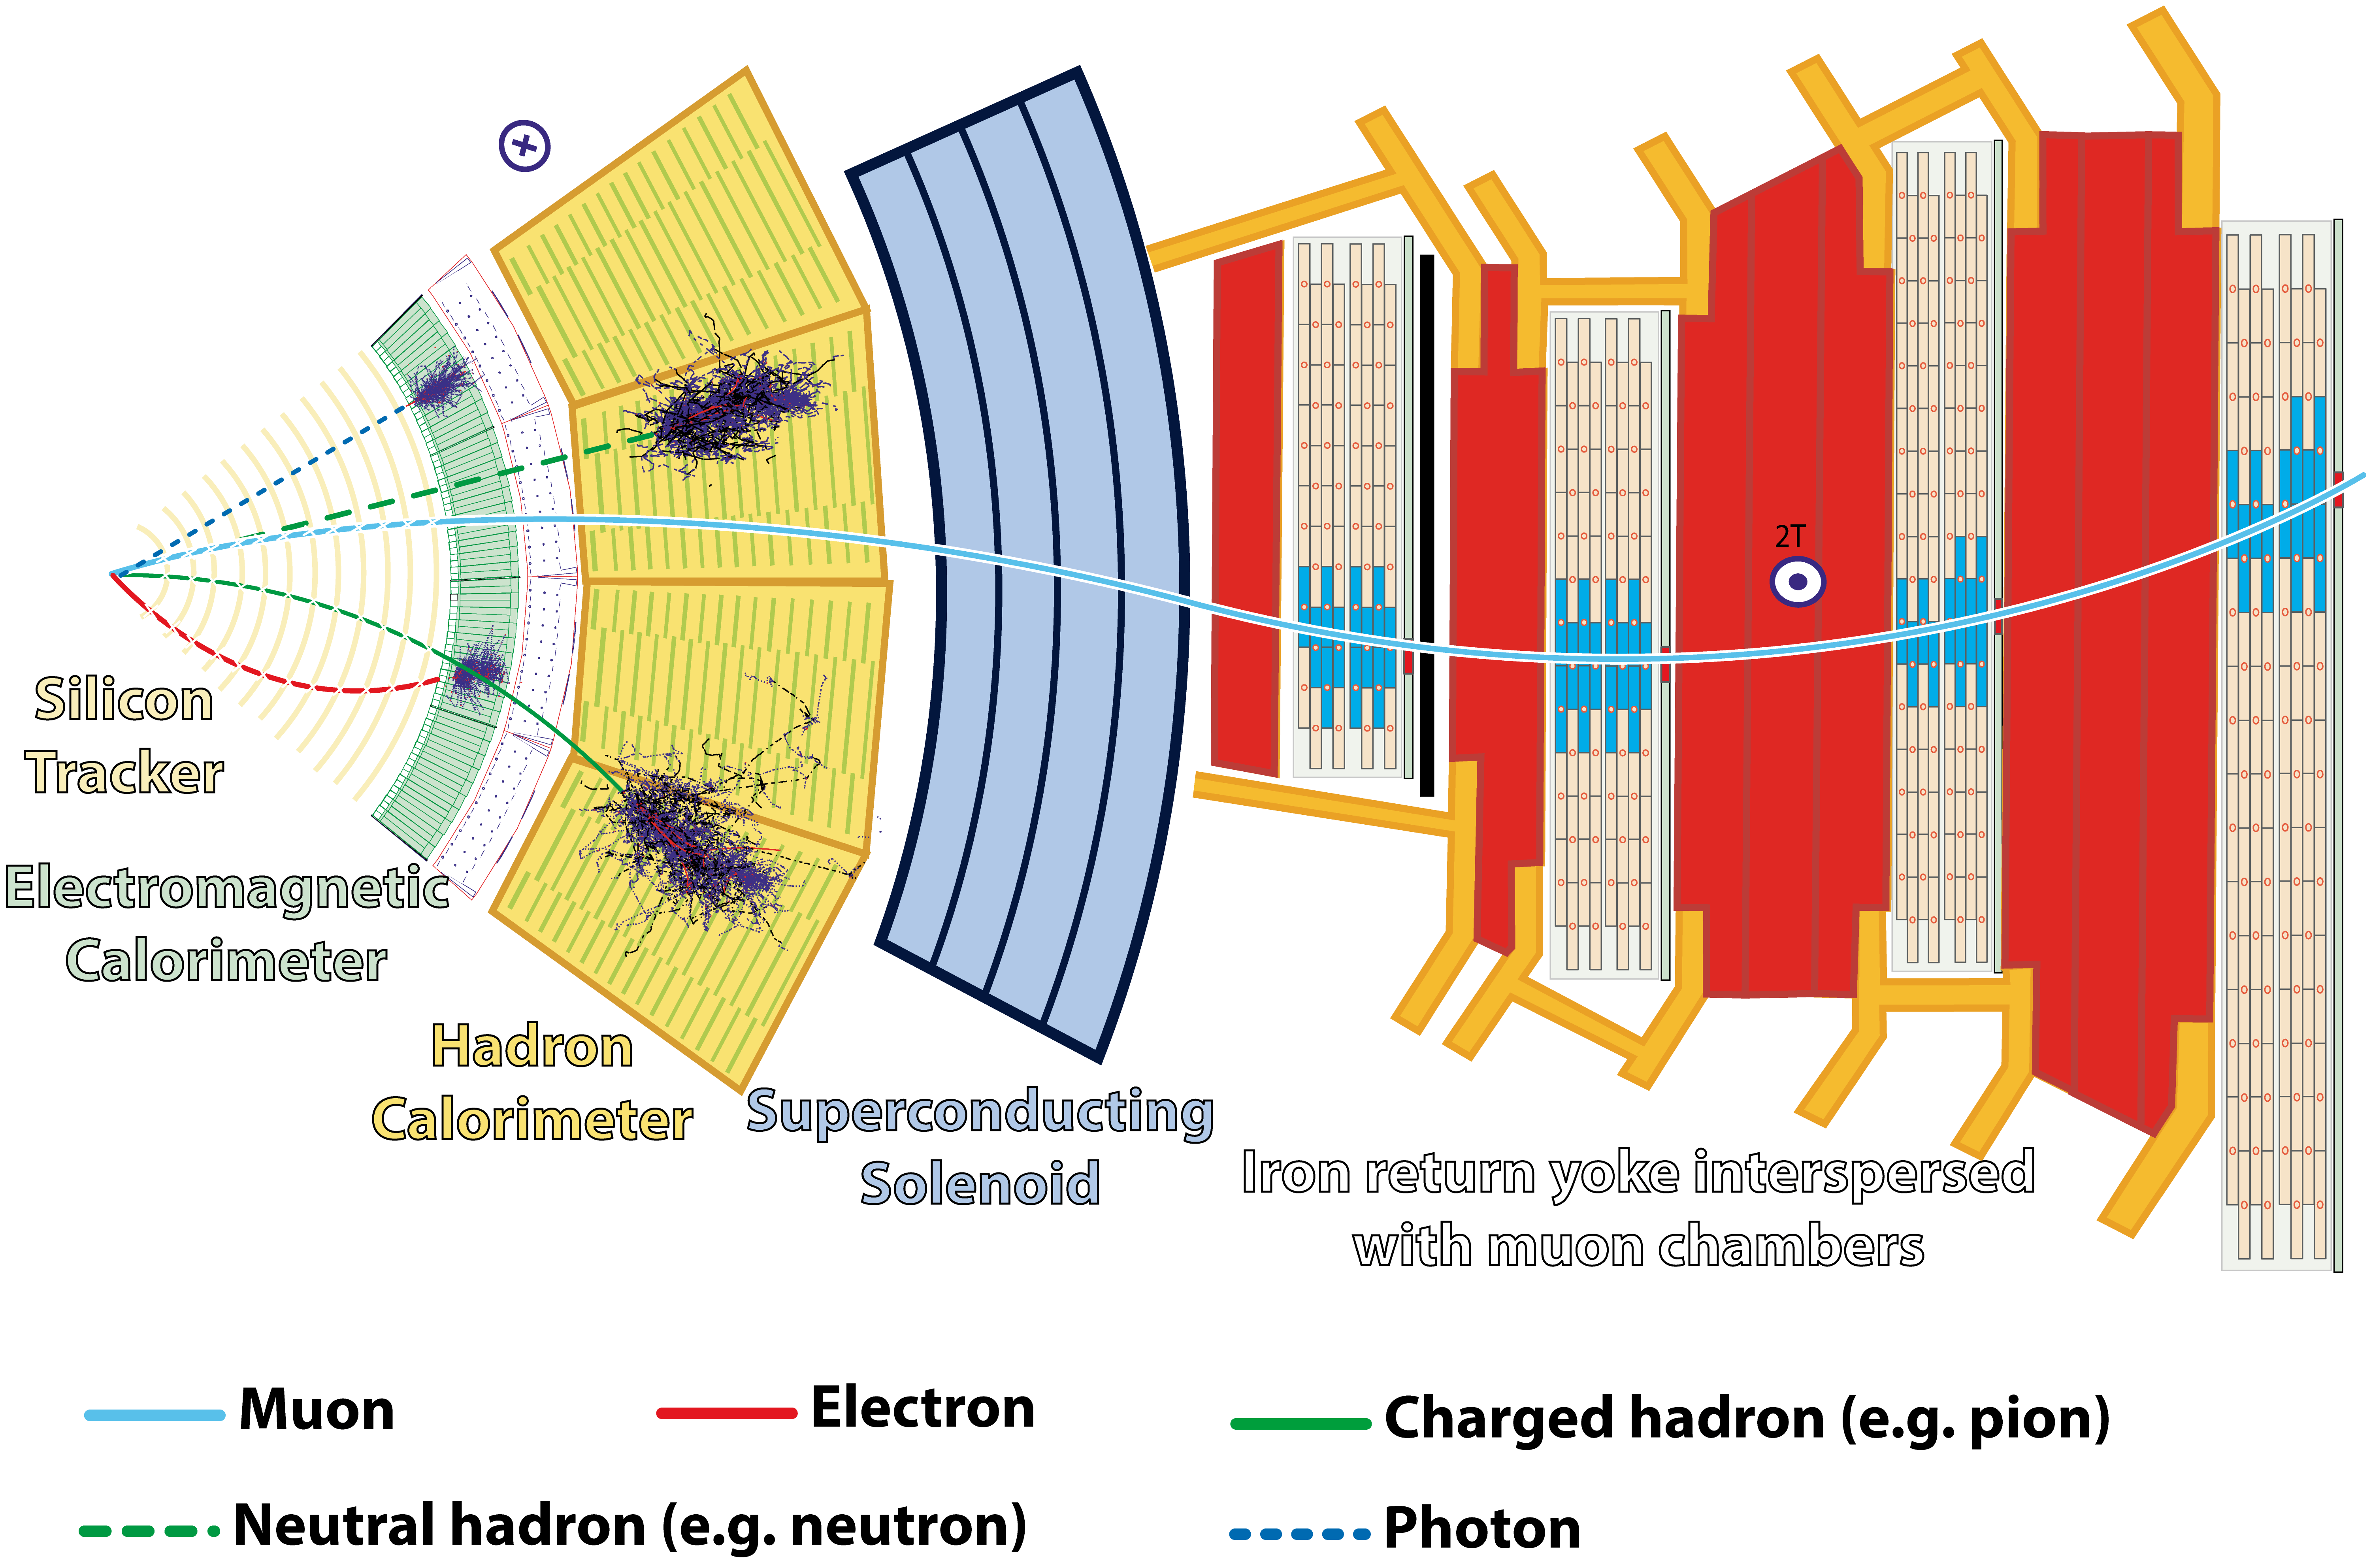
\includegraphics[width=0.85\textwidth]{Figures/CMSslice_whiteBackground.png}
\end{center}
\caption{A simplified transverse view of the CMS detector cross section \cite{CMS-PHO-GEN-2016-001}. The typical signatures of the five particle collections detected are shown.}
\label{fig:CMSslice}
\end{figure}

Within the solenoid volume there are three major subsystems.
A silicon pixel and strip tracker measures the trajectories of charged particles,
a lead tungstate crystal electromagnetic calorimeter (ECAL) mainly collects the energies of electrons and photons,
and a brass and scintillator hadronic calorimeter (HCAL) stops the more penetrating hadrons.
Quartz-fibre-based forward calorimeters further improve hermeticity.
The measurement of the muons properties relies on a combination of inner tracking and the information from the muon chambers,
which are gas-ionization detectors embedded in the steel flux-return yoke outside the solenoid.
A detailed description of the CMS detector can be found in Reference~\cite{CMS-CMS-00-001}.

\paragraph{Coordinate system\\}
CMS adopts a right-handed Cartesian coordinate system, with the origin defined in the centre of the detector; more precisely, the barycentre of the modules of the Tracker Outer Barrel.
The axes are oriented such that the x-axis points to the centre of the LHC ring, the y-axis is orthogonal to the LHC plane pointing up, and the the z-axis lies along the anticlockwise beam direction.

\paragraph{Kinematic variables\\}
In particle physics, the particle polar direction is often described with its rapidity, defined as:
\begin{equation}
  \label{eq:rapidityDefinition}
  y = \frac{1}{2} ln \frac{E + p_z}{E - p_z} \,.
\end{equation}

Difference in rapidity are invariant under Lorentz boosts along the z-axis.
In physics analyses the pseudo-rapidity is often used in its place, since the two coincide in the ultra-relativistic limit:
\begin{equation}
  \label{eq:pseudorapidityDefinition}
  \eta = - ln \left( \tan \frac{\theta}{2} \right) \,,
\end{equation}
where $\theta$ represents the polar angle with respect to the z-axis. The azimuthal angle, measured in the x-y plane is called $\phi$.
They are used to define a type of angular distance between two physical objects:
\begin{equation}
  \label{eq:deltaRDefinition}
  \Delta R = \sqrt{ \Delta \eta^2 + \Delta \phi^2 } \,.
\end{equation}

\subsection{Silicon tracker}
The CMS inner silicon tracker is the innermost subdetector of the CMS experiment, surrounding the interaction point, measuring 5.8 m in length and 2.5 m in diameter.
It provides precise measurement of the trajectories of the charged particles emerging from the LHC collisions.
These tracks are reconstructed by combining electrical signals (hits) from the outgoing charged particles as they traverse the tracker's layers.
Thanks to the uniform magnetic field within its volume, which bends the trajectories, it is able to provide accurate hits measurements,
allowing excellent reconstruction of the associated momentum and charge sign from the track parameters.

The accuracy of track reconstruction is crucial for determining the position of the hard scattering, the primary vertex, as well as in-flight decays resulting in secondary vertices.
This in turns allows for the suppression of the background from \pileup{} interactions,
which are simultaneous collisions between other pairs of protons in the same bunch crossing\footnote{
Strictly speaking, this is called in-time \pileup.
Collisions happening in the previous or next bunch crossing are referred to as out-of-time \pileup.
},
and a handle for measuring particle lifetimes.

The CMS tracker uses silicon pixel and strip sensors to cover $|\eta| < 2.5$, with a total area of $200\, \mathrm{m}^2$,
operating at temperatures of around -15\Celsius and -20\Celsius, respectively, to minimize the impact of the ionizing radiation damage.
To meet spatial measurement requirements amid particle flux, the finely segmented tracking detector with fast readout electronics minimizes the material to reduce multiple scattering.
Silicon's benefits include high charge carrier mobility, rapid signal processing, optimal energy resolution sensitivity, and excellent spatial resolution due to segmentation.
Local hit reconstruction involves clustering, noise calibration, and hit candidate conversion, providing cluster charge profiles and hit positions.

In 2017, the pixel detector underwent an upgrade, enhancing performances with additional layers in both barrel and endcaps \cite{CMS-TDR-11}.
The tracker's overall layout, shown in Figure \ref{fig:PIX_Phase_comparison}, optimally addresses the challenges posed by the LHC collisions.

The CMS tracker is structured in a hierarchical fashion, with a few large mechanical structures composed by smaller parts,
the smallest unit being always the single module.
A full overview of the structure hierarchies of the CMS tracker is shown in Figure \ref{fig:tracker_hierarchy}.

\begin{figure}
  \centering
  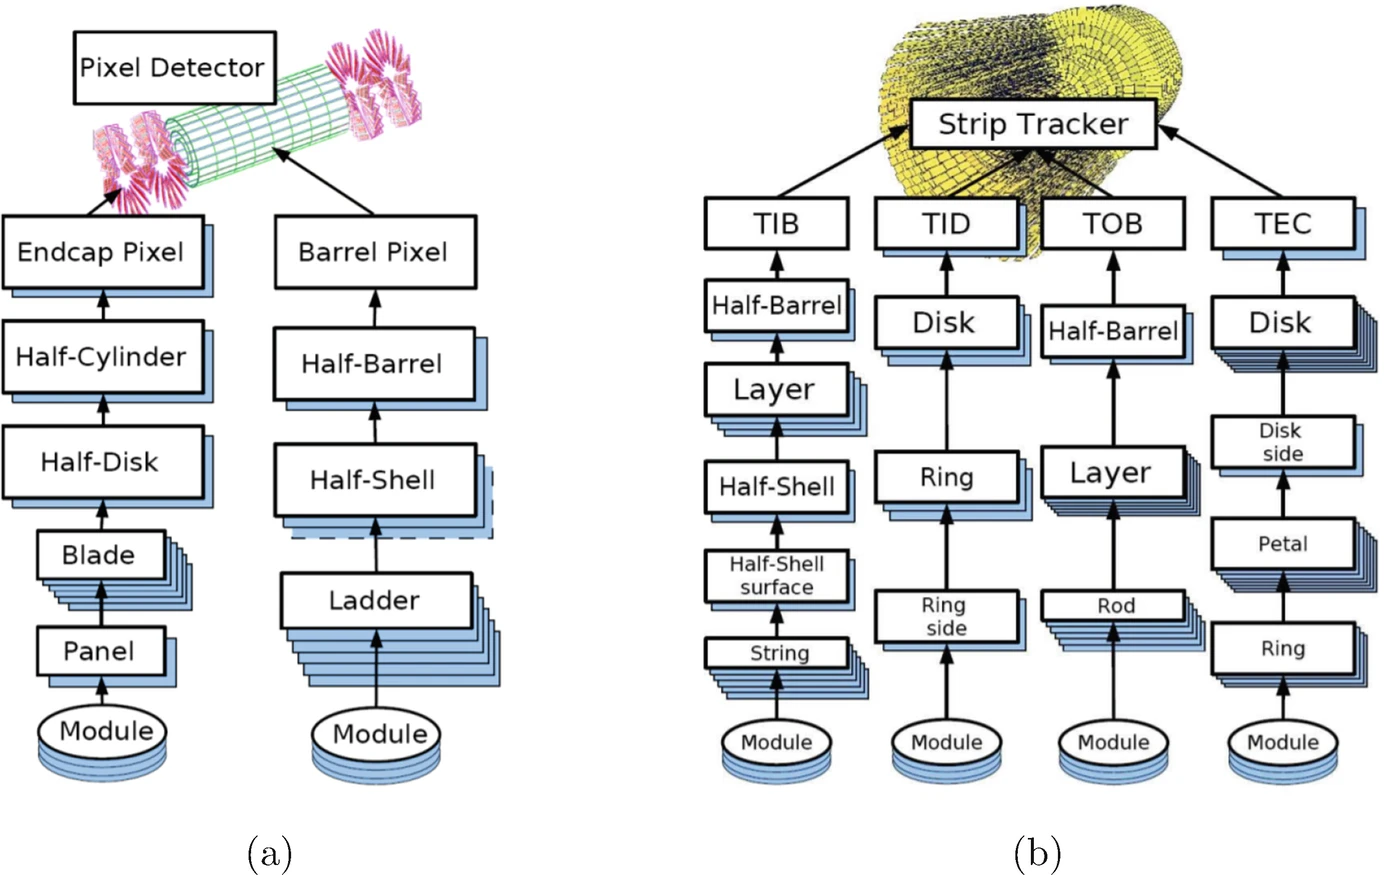
\includegraphics[width=0.85\textwidth]{tracker_hierarchy.png}
  \caption{Hierarchical structure of the CMS tracker, for the pixel (left) and for the strip (right) detectors \cite{CMS-NOTE-2009-002}.}
  \label{fig:tracker_hierarchy}
\end{figure}

\subsubsection{Silicon pixel detector}
The Pixel detector is the innermost tracking subsystem and it consists of two parts, the Barrel Pixel (BPIX) and the Forward Pixel (FPIX) detectors.
The description of the Phase-I pixel follows, and a comparison with the Phase-0 is shown in Figure \ref{fig:PIX_Phase_comparison}.

The BPIX is composed of four coaxial barrel layers located at a radial distance of 2.9, 6.8, 10.9 and 16.0\cm.
The FPIX consists of three endcap disks per side constituted by several blades positioned at a distance of 29.1, 39.6 and 51.6\cm from the nominal interaction point (IP).
The BPIX modules are parallel to the beamline, while the FPIX sensors are arranged into blades, oriented with a tilt of 20$\,^{\circ}$ with respect to normal incidence in order to exploit the Lorentz drift effect\footnote{
Charge carriers in the sensors, migrating along an electric field that is not parallel to the magnetic field, will have their trajectories deflected by a small angle $\theta_{LA}$.
This Lorentz drift effect broadens the charge cluster to neighbouring sensors (charge sharing), thereby improving the hit resolution.
}.

The 124 million pixels, around double the amount of the Phase-0 version, have an individual size of $100 \times 150 \mum^2$.
The front-end modules of the data acquisition (DAQ) system are powered by 1200 DC-DC converters that deliver the necessary voltage in the range of 2.4--3.3\usep V,
which were installed during the upgrade to cope with the increased number of channels while maintaining the existing cabling~\cite{Feld_2015}.
During the last period of data taking of 2017, called era F, 5\usep \% of the converter had failed and 35\usep \% were damaged (but working) due to the radiation damage aggravated by a design problem, and were successfully replaced during the 2017-2018 end-of-year technical stop~\cite{CMS:dcdc-failure-short}.

\begin{figure}[thb]
  \centering
  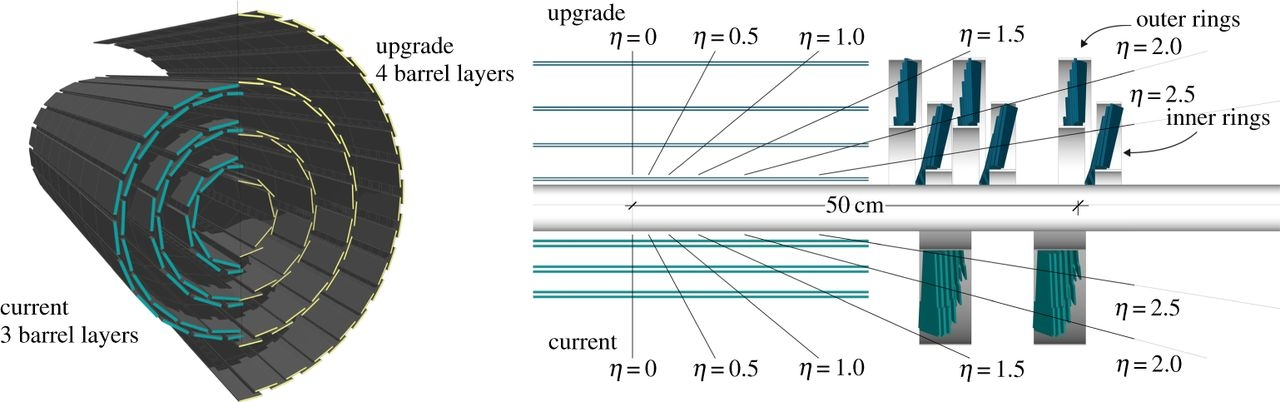
\includegraphics[width=0.85\textwidth]{PIX_Phase_comparison.jpg}
  \caption{A comparison of the different BPIX layers and FPIX disks between the Phase-0 and Phase-1 pixel detectors.}
  \label{fig:PIX_Phase_comparison}
\end{figure}

\subsubsection{Silicon strip detector}
The strip silicon tracker is located outside of the pixel detector at a radial distance comprised between 20 and 116 \cm.
It consists of 15148 silicon modules, with approximately 9.3 million strips and it extends over a pseudorapidity range up to $|\eta| < 2.5$.
The strip subsystem features an analogous barrel-endcap partition as in the case of the pixel detector.
The barrel region is subdivided into the Tracker Inner Barrel (TIB) and the Tracker Outer Barrel (TOB),
while the end-cap system is partitioned into the Tracker Inner Disks (TID) and the Tracker End Cap (TEC).

The inside of the tracker barrel is occupied by the four cylindrical layers of the TIB subdetector,
extending up to $\pm 65 \cm$ along the z axis, and the three TID disks covering up to a radius of $55 \cm$.
The double-sided modules arranged back-to-back present in the first two TIB layers allow for a hit measurement both in cylindrical coordinates
with a $23-34 \mum$ spatial resolution in the $r - \phi$ plane and of $530 \mum$ in the z-direction.
The TIB/TID system is enclosed by the six barrel layers of the TOB, which extends to a radius of $116 \cm$ and up to $\pm 118 \cm$ in the direction of the proton beam.
The TOB sensors are almost a factor two wider than the TIB due to the lower particle fluence.
Coverage in the z region $124 \le |z| \le 282 \cm$ is ensured by the TEC subdetector, composed of nine disks of various sizes,
providing hit positional information in the $r - \phi$ plane with a resolution in the range $18 - 47 \mum$.

\subsection{Electromagnetic calorimeter}
The Electromagnetic Calorimeter (ECAL) \cite{CERN-LHCC-97-033} provides a measurement of the energy of incoming electrons and photons.
It is a hermetic, homogeneous calorimeter made of scintillating crystals of lead tungstate ($\mathrm{PbWO_4}$).
The material was chosen because of its short radiation length (0.89\cm) and high density,
which allow the absorption of electromagnetic showers within the short length;
its small Moli\`ere radius (2.2\cm) allows a good shower separation.
Its response time is fast, and 80 \% of the scintillation light is emitted within the 25 ns between the LHC bunch crossings.
The general structure is shown in Figure \ref{fig:ECAL_3D_colour}.

\begin{figure}[thb]
  \centering
  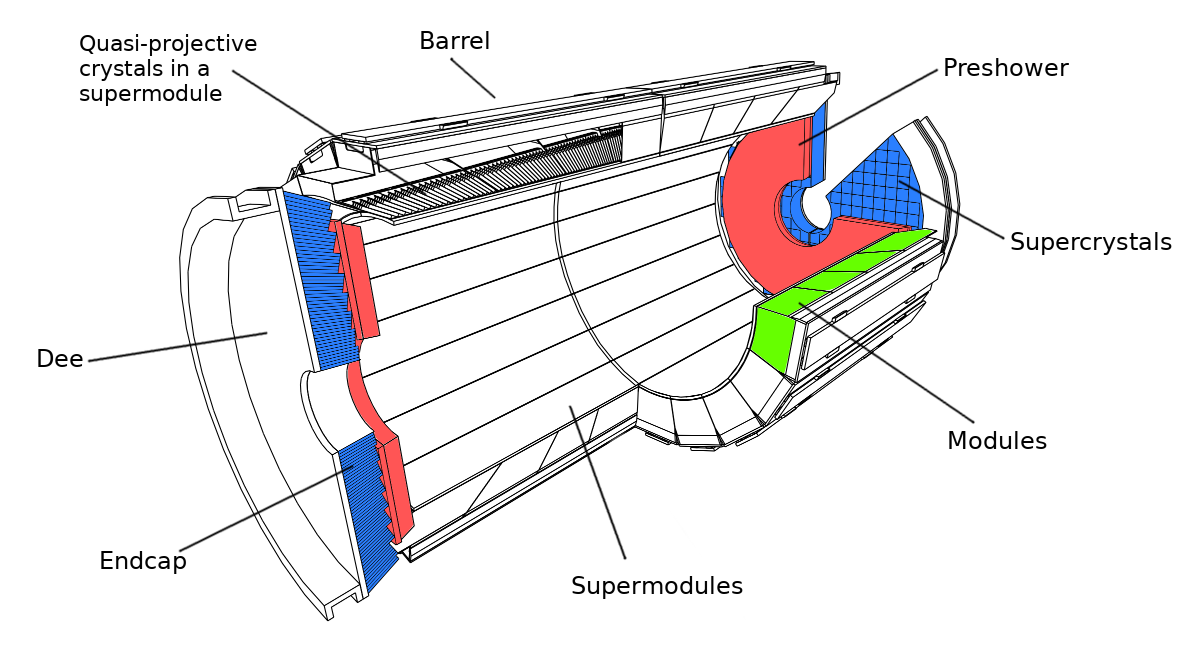
\includegraphics[width=0.85\textwidth]{ECAL_3D_colour.png}
  \caption{A 3D render of ECAL with the main components highlighted \cite{siddireddy2018cms}.}
  \label{fig:ECAL_3D_colour}
\end{figure}

ECAL is composed of Electromagnetic Barrel (EB), Electromagnetic Endacp (EE) and Endcap Preshower (PS).
EB is made of 61200 crystals with a quasi-projective geometry, and each endcap has 7324 crystals.
The EB has an inner radius of $129 \cm$, and it is structured as 36 identical ``Supermodules'',
each covering $20\usep ^{\circ}$ in $\phi$ and half the barrel length, corresponding to a pseudorapidity interval of $0 < |\eta| < 1.479$.
Each supermodule contains four modules with 400 or 500 crystals apiece, each with a length of 230 mm and a cross section of $22 \times 22 \usep \mathrm{mm}^2$.
The EE is at a distance of $314 \cm$ from the vertex and covering a pseudorapidity range of $1.479 < |\eta| < 3.0$,
and is made of crystals with a length of 220 mm and a cross section of $28.62 \times 28.62 \usep \mathrm{mm}^2$.

The crystals have a quasi-projective geometry, with an angle of 3$\usep ^{\circ}$ from the nominal interaction point in both $\theta$ and $\phi$ directions,
to avoid the alignment of inter crystal gaps with particle trajectories.

The scintillation light from ECAL crystals is read by fast, radiation-tolerant photodetectors which can operate inside the CMS magnetic field
and are insensitive to particles traversing them.
Two preshower detectors are installed at each end of the tracker detector, in front of the ECAL endcaps,
in order to help distinguishing $\Pgpz \to \PGg \PGg$ decays from single photons and identifying electrons against minimum ionizing particles.
These sampling calorimeters are made of a lead radiator layer which initiates electromagnetic showers from incoming particles,
followed by silicon strip sensors that measure the deposited energy.
Although lead tungstate crystals are radiation resistant, they undergo a limited but rapid loss of optical transmission under irradiation.
This phenomenon depends on the luminosity and crystal pseudorapidity, and is partly balanced by an annealing effect.
This effect is measured and it is taken into account by time-dependent corrections applied to the measured particle energies.

The ECAL energy resolution $\sigma_E/E$ for electrons was obtained in a test beam measurement \cite{CMS-NOTE-2006-148}, and has the following energy dependency:
\begin{equation}
  \frac{\sigma_E}{E} = \frac{2.8\%}{\sqrt{E\, [\GeV]}} \oplus \frac{12\%}{E\, [\GeV]} \oplus 0.3\% \,,
\end{equation}
where the $\oplus$ symbol denotes the sum in quadrature of the individual contributions.
The first term represents the stochastic part which dominates for energy deposits of photoelectrons below 100\GeV;
the second term stands for the noise contribution;
the constant accounts predominantly for calibration inaccuracies and additionally for the non-uniform response of the photodetectors.

\subsection{Hadronic calorimeter}
The HCAL calorimeter is a sampling detector employed for the measurement of the energy deposits of hadrons.

The central part of the HCAL covers a pseudorapidity range up to $|\eta| < 1.3$ and it consists of two distinct subdetectors:
the inner barrel (HB) part with brass absorbing layers and plastic scintillator tiles,
and the outer hadronic calorimeter (HO) entirely composed of plastic scintillators, installed outside the solenoid.
Because of the limitations in size of the CMS calorimeter, some of the most-energetic hadronic tails may leak outside the full volume of the HB detector.
Thus, the HO subdetector has been installed to extend the depth of the HCAL to 11.8 hadronic interaction lengths
in order to catch the most energetic hadronic shower tails, utilizing the magnet coil as an absorber.

The HCAL endcaps (HE) cover the range $1.3 < |\eta| < 3$ and uses the same brass absorber as HB.
It is required to handle high counting rates and have high radiation tolerance.
Including the EB in front of it, it has a total depth of around 10 interaction lengths.
The scintillation light produced by plastic tiles is collected by wavelength shifting fibres and detected by multipixel hybrid photodiodes.

The hadron forward calorimeter (HF) extends the pseudorapidity range to $|\eta| = 5.2$ and it is located at a distance of 11\usep m from the beamspot.
Since it is affected by hadronic energy depositions seven times more intense than in the rest of the HCAL,
it is composed of iron absorbers and quartz fibre as active material, due to their higher more radiation-hardness.
It is further equipped with a set of photomultipliers, which detect the cone of Cherenkov light emitted by charged particles passing through the material.

The segmentation of the tiles is $\Delta \eta \times \Delta \phi = 0.087 \times 0.087$ for $|\eta| < 1.6$ and $\simeq 0.17 \times 0.17$ for $|\eta| \ge 1.6$.

%% The relative HCAL energy response curve for isolated charged pions is illustrated in Figure 2.8.
%% A broader response curve is an indicator of a larger \pileup{} contamination.
%% Out-of-time \pileup{} mitigation helps reduce the latter, thereby improving the quality of pion isolation.
HCAL is instrumental in recognizing hadrons and their decay products,
and provides a crucial measurement of the missing transverse energy exploiting its extensive coverage in $\eta$, a property referred to as hermeticity.
The HF is also used for two of the methods for measuring the instantaneous luminosity.

\begin{figure}[thb]
  \centering
  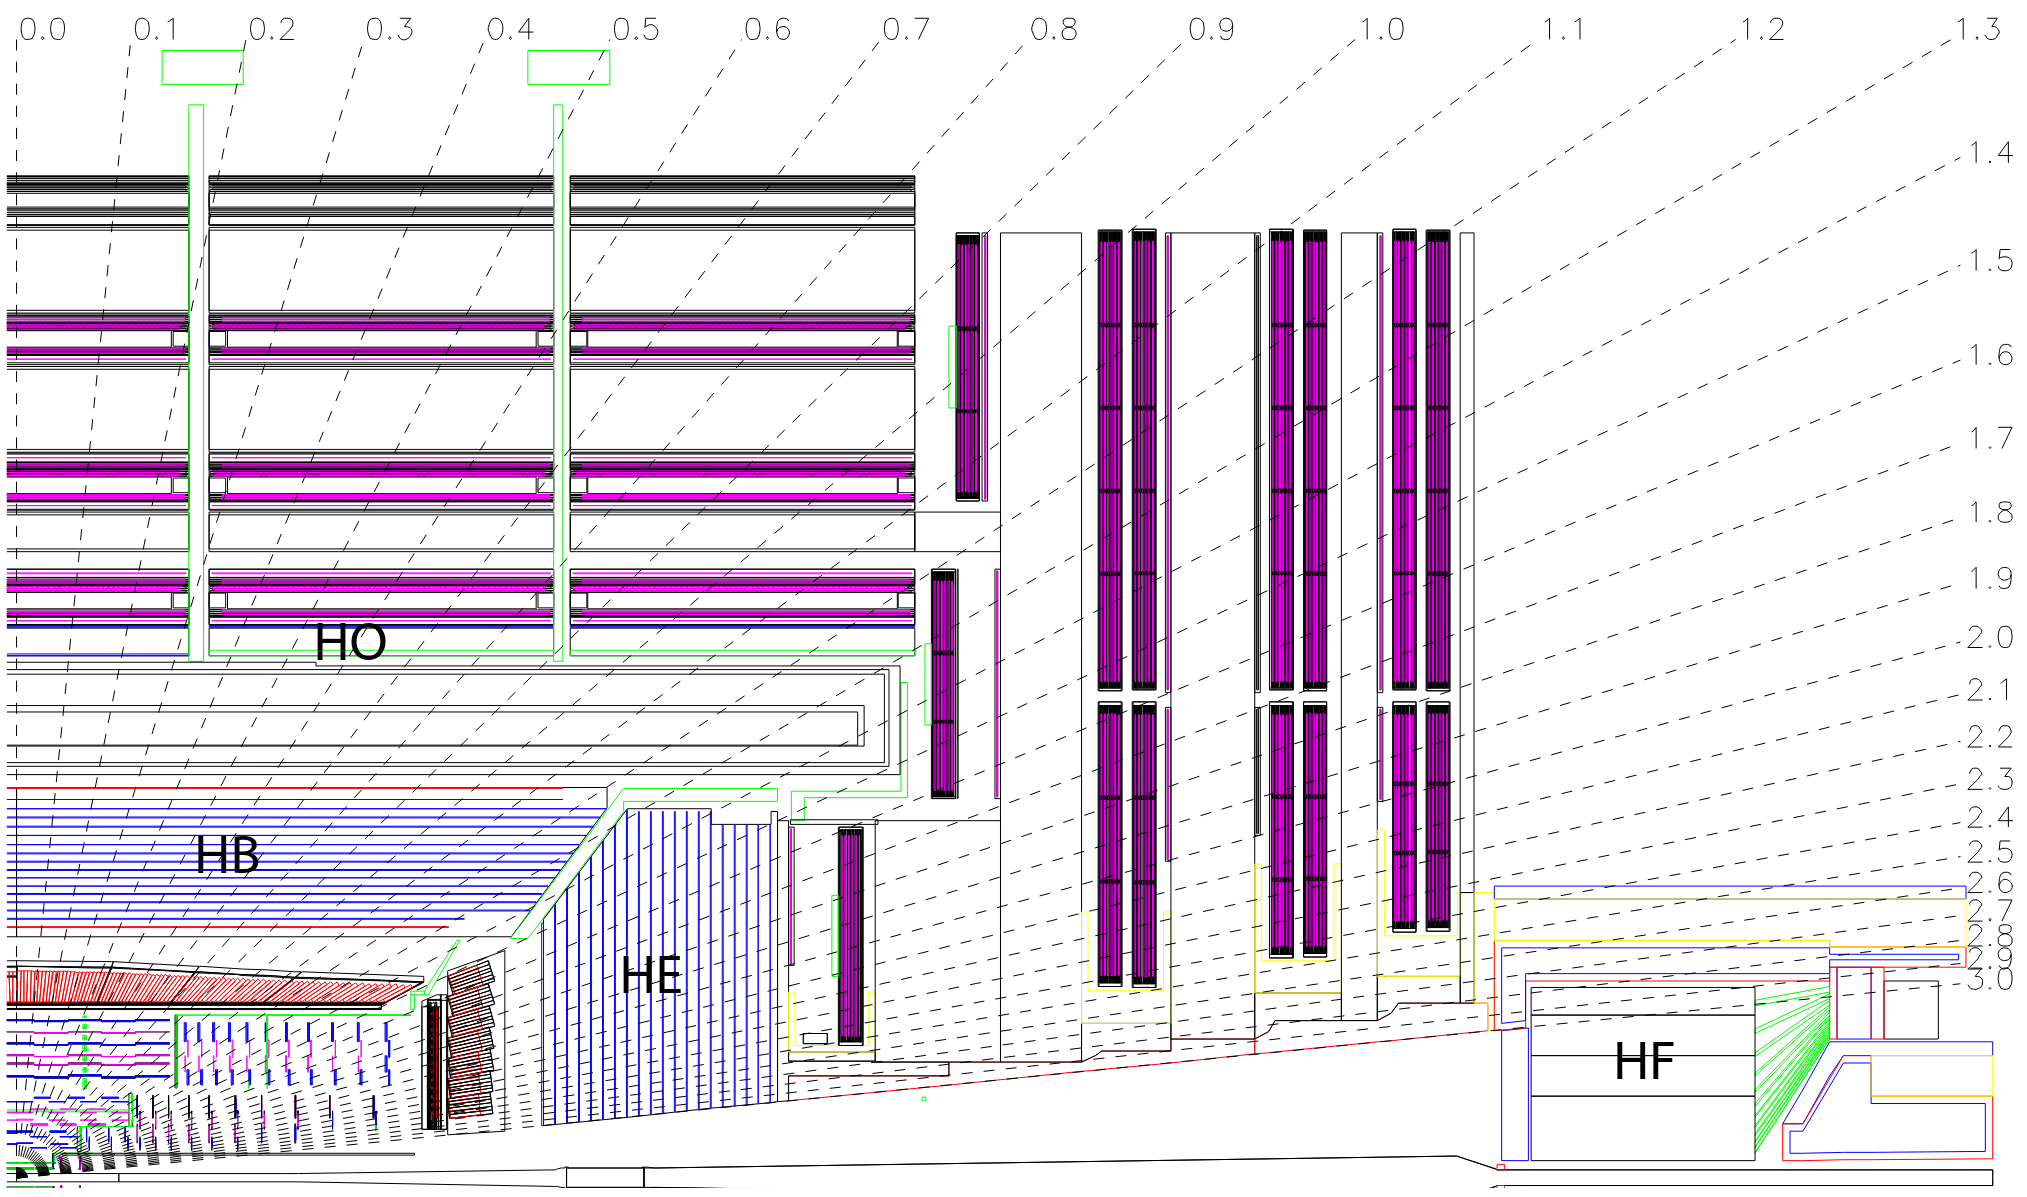
\includegraphics[width=0.85\textwidth]{HCAL_2Dquarter.png}
  \caption{Longitudinal view of the CMS detector showing the locations of the hadron barrel (HB), endcap (HE), outer (HO) and forward (HF) calorimeters. \cite{CMS-CMS-00-001}.}
  \label{fig:HCAL_2Dquarter}
\end{figure}

\subsection{The muon system}
Muons produced in collisions at the LHC usually traverse the Tracker, ECAL, HCAL,
and the solenoid volumes without being stopped and are identified and measured in the muon detectors located in the outermost part of CMS.
The muon system is made of muon chambers embedded in the iron return yoke of the CMS magnetic field
and is divided into a cylindrical barrel section and two planar endcaps.
It uses three types of gas-ionization chambers: Drift Tubes (DT), Cathode Strip Chambers (CSC) and Resistive Plate Chambers (RPC).
A new set of muon detectors using the Gas Electron Multiplier (GEM) technology
and designed to cope with the foreseen increased luminosity of HL-LHC is being installed in the endcap section~\cite{CMS-TDR-013}.
The layout of the three subsystems is shown in Figure \ref{fig:MUON_2Dquarter}.

\begin{figure}[thb]
  \centering
  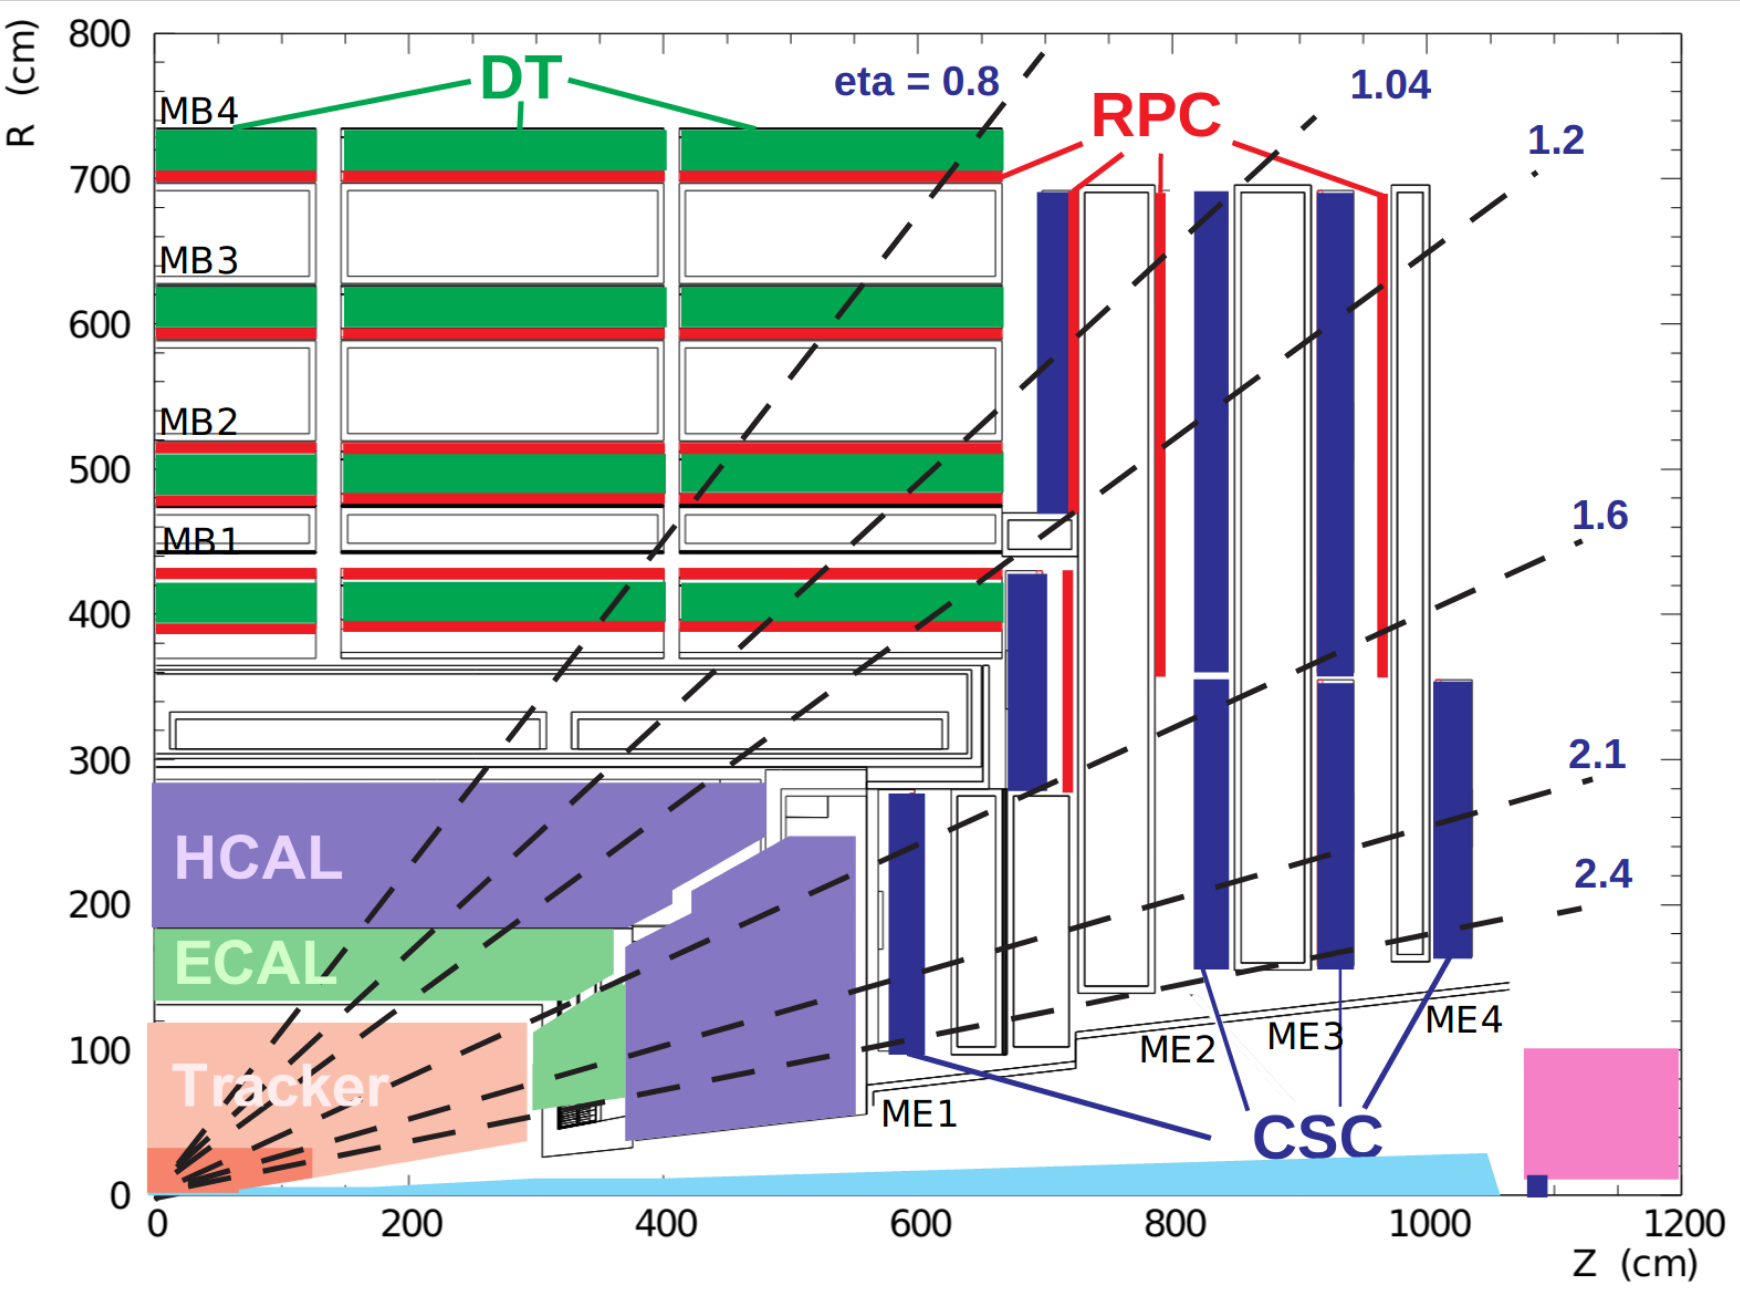
\includegraphics[width=0.85\textwidth]{MUON_2Dquarter.png}
  \caption{Longitudinal layout of one quadrant of the CMS detector.
    The four DT stations in the barrel (MB1–MB4, green),
    the four CSC stations in the endcap (ME1–ME4, blue),
    and the RPC stations (red) are shown~\cite{CMS-MUO-10-004}.}
  \label{fig:MUON_2Dquarter}
\end{figure}

\subsubsection{Drift Tubes}
The Drift Tubes (DTs) are located in the barrel region, where the muon rate is lower and the magnetic field is quite uniform,
and cover a pseudorapidity range of $|\eta| < 1.2$.
The DTs are organized into four stations interspersed among the layers of the flux return plates.
Their basic constituents are rectangular drift cells bounded by two parallel aluminium planes, which serve as cathodes.
Anodes are 80\mum stainless steel wires located in the centre of each cell.
A muon passing through a cell ionizes the gas mixture that fills the cell volume.
The drift time of the resulting electrons is then used to measure the distance between the muon track and the wire.
Each chamber has a resolution of 100 µm in the $r - \phi$ plane.

\subsubsection{Cathode Strip Chambers}
The Cathode Strip Chambers (CSCs) are used in the endcaps, where the the muon rates and background levels are higher and the magnetic field is large and non uniform,
and cover a pseudorapidity range of $0.9 < |\eta| < 2.4$.
The CSCs are multiwire proportional chambers, made of 6 anode wire planes interleaved among 7 cathode panels,
with the wires running approximately perpendicular to the strips.
A muon passing through a chamber generates an avalanche, inducing a charge on several cathode strips.
The ensuing interpolation allows a spatial resolution of 50\mum to be obtained.
Four stations of CSCs are located in each endcap.
The chambers are positioned perpendicular to the beam line and interspersed between the magnetic field flux return plates.

\subsubsection{Resistive Plate Chambers}
The Resistive Plate Chambers (RPCs) are located both in the barrel and in the endcaps and cover the pseudorapidity range $|\eta| < 1.6$.
The RPCs are double-gap chambers which operate in avalanche mode and are disposed in six layers in the barrel and three layers in the endcaps.
They provide a complementary trigger system with moderate spatial resolution but excellent time resolution (of the order of 1 ns),
which helps measuring the correct beam-crossing time.

\subsubsection{Gas Electron Multiplier}
A Gas Electron Multiplier (GEM) consists of a layer of electrically insulated polymer coated with metal and chemically perforated.
A significant voltage is applied between the two metal sides, which results in high electric fields inside the holes,
where electons produced by an ionizing particle in the gas produce an electron avalanche.
A GEM chamber has multiple layers (3 for the ones used in CMS).
A demonstrator, consisting of 144 chabers, has already been installed during Long Shutdown~2 (2019--2021),
after the end of \Run2 and is currently contributing to the \Run3 data taking.

\subsection{Trigger system}
The enormous LHC proton-proton collision rate of 40 MHz with a characteristic event size of approximately 1 MB
is a serious challenge to the CMS Data Acquisition (DAQ) system.
However most of the data refers to low-energy interactions, rather than hard scattering and rare processes.
Thus the need for a system that is able to reduce the huge data flow to a manageable rate prior to storage on disk,
whilst selecting efficiently the interesting events is necessary.
These requirements are met by the so-called CMS triggering system,
which reduces the initial bandwidth by over three orders of magnitude.
The CMS triggering system adopts a sophisticated two-stage approach,
consisting of a \Lone trigger (L1) fully implemented in hardware logic and a high-level trigger (HLT) software farm.
%% The L1 trigger achieves a rate reduction down to the level of 100 kHz, which is subsequently downscaled to around 1 kHz at HLT level.

\subsubsection{Level-1 Trigger}
\label{sec:L1trigger}
The L1 trigger achieves a rate reduction down to the level of 100 kHz, with a latency below 4\mus.
It is implemented in custom hardware, using Field Programmable Gate Arrays (FPGAs) which are generic and easily customizable,
and Application Specific Integrated Circuits (ASICs), which are more resilient to high \pileup{} conditions, albeit not easily reconfigurable.
The \Lone trigger uses information from the calorimeters and the muon system to construct the so called \textit{trigger primitives},
which are the base of the trigger logic.
An overview of the layout of the system is shown in Figure \ref{fig:L1trigger-block-diagram}.

\begin{figure}[thb]
  \centering
  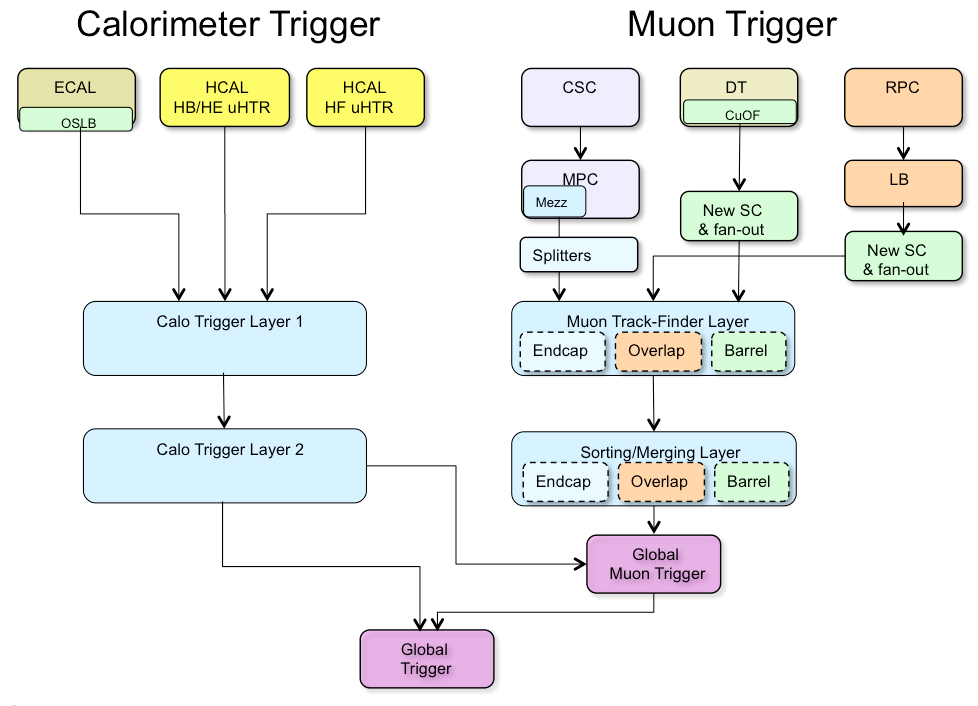
\includegraphics[width=0.85\textwidth]{L1trigger-block-diagram.png}
  \caption{Main data-flow diagram for the Phase-1 \Lone trigger \cite{CMS-TDR-12}.}
  \label{fig:L1trigger-block-diagram}
\end{figure}

\subsubsection{High-level Trigger}
The High Level Trigger (HLT) is a sophisticated software-based system which uses tens of thousands of CPU cores
running multithreaded instances of an optimized version of the CMS reconstruction algorithm~\cite{CMS-TRG-12-001}.
This array of commercial CPUs manages the full event reconstruction through several sequential algorithms,
targeting signature of interest referred to as \textit{trigger path}.
The goal of the HLT is to reduce the incoming \Lone rate of 100 kHZ to around 1 kHz,
while maintaining a good efficiency in the various phase spaces of interest for physics
and being as inclusive as possible to enable a broad variety of searches.

For this purpose, some paths that would otherwise exceed the available bandwidth are made to only pass the selection after a pre-scale.
This consists of a random discarding of the event, either at L1 or at HLT, which is then accounted for in the analysis.

Another major constraint of the HLT is the maximum processing time for each event, which is 50 ms.
To optimize it, the more computationally-intensive algorithms are run at the end of the filtering sequence.
These modules perform a streamlined version of the standard offline reconstruction.
